\section{Результати виконання роботи}

Для підтвердження коректності роботи розробленої ієрархії класів, перевірки 
працездатності абстрактних методів та демонстрації динамічного поліморфізму 
через інтерфейсні типи посилань було виконано компіляцію та запуск коду. 
Компіляція та виконання програми здійснювалися в терміналі PowerShell середовища 
розробки VS Code з примусовим встановленням кодування UTF-8.

На рисунку \ref{fig:terminal_output} представлено скріншот вікна терміналу з 
результатами виконання програми.

\begin{figure}[H]
    \centering
    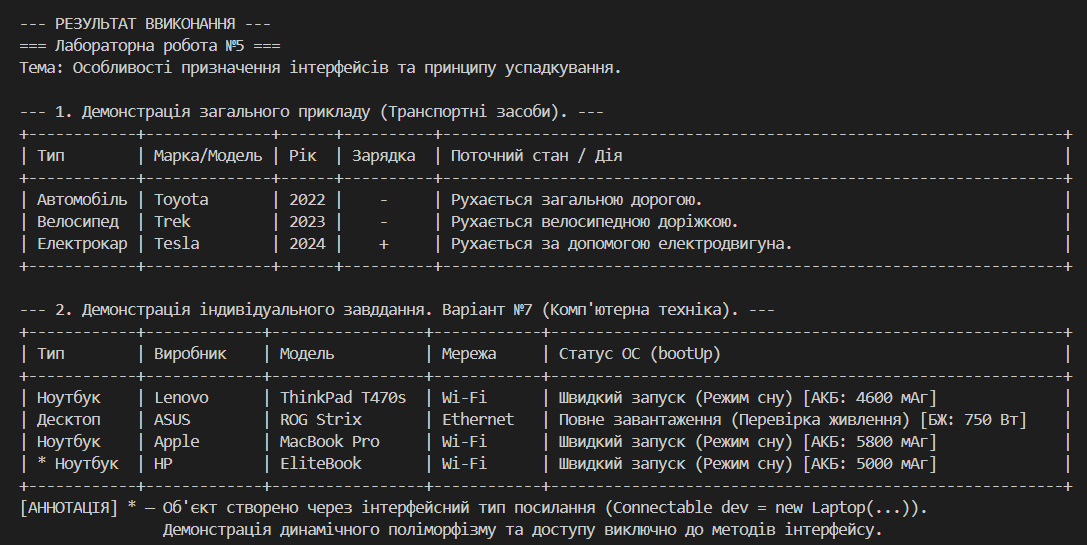
\includegraphics[width=0.95\textwidth]{screenshots/terminal_output.png}
    \caption{Скріншот результатів виконання програми в терміналі VS Code завдання лабораторної роботи №5}
    \label{fig:terminal_output}
\end{figure}

Завдяки винесенню логіки форматування в головний клас \texttt{Main.java} було реалізовано 
принцип розділення відповідальності. Дочірні класи не містять 
елементів CLI-розмітки, повертаючи виключно інформаційні рядки стану, що дозволяє гнучко 
масштабувати систему та змінювати формат представлення даних без рефакторингу бізнес-логіки 
ієрархії.